\documentclass[10pt,twocolumn]{article}
\usepackage[a4paper,margin=17mm,columnsep=6mm]{geometry}
\usepackage[T1]{fontenc}
\usepackage[utf8]{inputenc}
\usepackage[expansion=false]{microtype}
\usepackage{booktabs}
\setlength{\tabcolsep}{3.5pt}
\usepackage{titlesec}
\titlespacing*{\section}{0pt}{1.4ex plus .5ex}{0.6ex}
\titlespacing*{\subsection}{0pt}{1.0ex plus .4ex}{0.4ex}
\usepackage{graphicx}
\usepackage{amsmath}
\usepackage{xcolor}
\usepackage[hidelinks]{hyperref}
\usepackage{natbib}
\bibliographystyle{plainnat}

\title{Capability Is Not Behaviour: A Capability-Conditioned Audit of a Multi-Agent Transaction Pipeline and a Regulatory GraphRAG Assistant}
\author{Abhilash Reddy Maram\\ \small Independent researcher, Offenburg, Germany\\ \small \texttt{persistentlearningsys@gmail.com}}
\date{October 2026 --- technical report}

\begin{document}
\maketitle

\begin{abstract}
Agentic LLM systems are usually evaluated on end-to-end task success, which cannot tell a missing capability from a capability that is present but not applied. Following the capability-conditioned view of goal-directedness of \citet{everitt2025goal}, I evaluate two systems I built for regulated finance: \textsc{FinStream}, a three-agent transaction pipeline (deterministic PII sanitiser, retrieval-augmented classifier, graph-augmented fraud detector), and a GraphRAG assistant over 11 EU financial regulations. For \textsc{FinStream} I score each agent in isolation on 400 labelled transactions across five stress conditions, score the full chain on the same transactions, and attribute every end-to-end failure to a component and to whether that component succeeded alone. The audit exposed a design defect that no single-agent test can see: the sanitiser's output was never handed to the LLM agents, so 100\% of records reached an external model with raw PII (1{,}656 identifiers) although the system's documentation claimed otherwise; only 1\% of output records echoed it, so an output-only audit would have passed the system. A deterministic hand-off fix removes the exposure entirely at zero task cost. The remaining failures are almost all retrieval-layer: a Cypher traversal that cannot follow mixed-relationship paths silently cleared two of three second-hop fraud-ring members in 100\% of cases. For the assistant I compare vector RAG, GraphRAG and a closed-book baseline on 125 questions with article-level ground truth. The base model answers 74\% of questions correctly without any documents, so headline RAG accuracy (76\%) overstates retrieval's contribution; retrieval-dependent accuracy is 26\%, and what retrieval actually buys is precision (hallucinated specifics 29.5\%\,$\to$\,9.5\%). 18 of 25 RAG failures occurred with the gold passage already in context, most through dates imported from a neighbouring regulation. I argue that scoring subtasks and composites on the same inputs, together with contamination-resilient question sets, is the right unit of safety evaluation for deployed agent systems, and outline verifiable hand-off contracts as the generalisation of the fix.
\end{abstract}

\section{Introduction}
\label{sec:intro}

Foundation models are increasingly deployed as components of pipelines: one agent redacts, another retrieves and classifies, a third reasons over a graph. The usual evaluation reports a single end-to-end success rate. That number conflates two different failure modes. A \emph{capability gap} means a component cannot do its subtask. A \emph{goal-directedness deficit}, in the sense of \citet{everitt2025goal}, means the components can do their subtasks but the system does not apply those capabilities towards the overall goal. The remedies differ: the first needs better models or more data; the second needs better composition, and is often fixable deterministically.

\citet{everitt2025goal} measure this distinction for single LLMs on synthetic tasks, using subtasks to estimate capability and composite tasks to estimate how much of that capability is used. This report applies the same logic to two systems I built in early 2026, in a domain where the goal that matters most---personal data must not reach an external model---is exactly the kind of goal end-to-end accuracy does not measure:
\begin{itemize}\setlength\itemsep{1pt}
  \item \textsc{FinStream}: a Kafka-driven pipeline with a deterministic PII sanitiser (Agent~1), a pgvector-RAG semantic classifier (Agent~2) and a Neo4j GraphRAG fraud detector with a circuit breaker (Agent~3), on Spring~AI with Claude Haiku~4.5.
  \item A GraphRAG knowledge assistant over 11 EU regulations (PSD2, SCA RTS, SEPA, MiCA, DORA, EMD2, AMLD5/6, GDPR, IFR; 2{,}393 chunks) with a small knowledge graph of providers, regulations and requirements, on the same model.
\end{itemize}

\paragraph{Contributions.}
(1)~A capability-conditioned evaluation protocol for agent pipelines: isolated subtask scores, composite scores on the same inputs, and per-failure attribution into \emph{capability absent} vs.\ \emph{capability present, not applied}.
(2)~A hand-off audit that found and quantified a PII exposure in a pipeline whose documentation claimed PII was masked before any LLM call, and a deterministic fix evaluated under the same protocol.
(3)~A 125-question regulatory QA set with article-level ground truth and a 20-question unanswerable subset, used with a closed-book baseline to separate retrieval from parametric recall.
(4)~Measured effects of four stress conditions (PII in free text, obfuscated PII, out-of-distribution merchants, prompt injection), including a null result.
Code, data, harnesses and raw results are public.\footnote{\url{https://github.com/plsyz/finstream-ai} and \url{https://github.com/plsyz/fintech-knowledge-assistant}, branches \texttt{eval/*}.}

\section{Related work}
\label{sec:related}

\paragraph{Goal-directedness and capability-conditioned evaluation.}
\citet{everitt2025goal} define goal-directedness as the extent to which a model uses its capabilities towards a given goal and show it differs from task performance and is only moderately sensitive to motivational prompts. I borrow the construction (subtasks estimate capability; composites estimate use) and move it from a single model to a pipeline, where the ``composition'' is explicit code rather than in-context reasoning, which makes the attribution exact.

\paragraph{Interpretable, sample-efficient alignment.}
HyPerAlign \citep{garbacea2025hyperalign} replaces preference fine-tuning with explicit, inspectable hypotheses that steer generation in context. The fix evaluated here is in the same spirit at the system level: an inspectable, deterministic contract on what each agent may see, rather than a retrained model.

\paragraph{Evaluation that resists aggregation and contamination.}
\citet{garbacea2026personalized} show that aggregate benchmark rankings hide per-user disagreement; the present work shows that aggregate end-to-end scores hide per-component and per-merchant disagreement. \citet{sainz2023contamination} argue that LLM evaluation must measure data contamination; the closed-book baseline in Section~\ref{sec:kb} is a lightweight version of that check for RAG systems.

\paragraph{RAG grounding and LLM judges.}
RAG \citep{lewis2020rag} and GraphRAG \citep{edge2024graphrag} are evaluated here on citation and support rather than fluency, following faithfulness-style metrics \citep{es2024ragas,min2023factscore}; the judge protocol follows \citet{zheng2023judge} with a model distinct from the system under test.

\paragraph{Prompt injection and systems safety.}
Indirect prompt injection through data fields \citep{greshake2023injection} motivates the \texttt{prompt\_injection} condition. The distinction between a component that works and a system that works is the founding observation of systems-safety engineering \citep{leveson2011}; my aeronautical engineering background is where I first met it, and this protocol is an attempt to make it measurable for LLM pipelines.

\section{Capability-conditioned evaluation of \textsc{FinStream}}
\label{sec:finstream}

\subsection{System and the hand-off defect}
Agent~1 masks four structured fields (name, account number, e-mail, IP) with regular expressions. Agent~2 builds a query from merchant, description and MCC, retrieves five similar labelled transactions from pgvector and asks the LLM for one of eleven categories. Agent~3 runs a two-hop Cypher traversal over \texttt{SHARES\_IP\_WITH}, \texttt{SHARES\_ADDRESS\_WITH} and \texttt{PREVIOUSLY\_FLAGGED\_IN}, formats the subgraph into the prompt and asks for a risk level, a flag and an evidence-citing reason. An orchestrator chains them and emits a processed record.

Reading the orchestrator for this evaluation showed that Agents~2 and~3 were called with the \emph{raw} transaction. Agent~1's output was only assembled into the final record. The system therefore passed every single-agent test of the sanitiser while violating the pipeline's stated goal. I kept this behaviour as the \texttt{raw} hand-off mode and added a \texttt{sanitized} mode in which the LLM agents receive the masked fields plus a scrubbed description (e-mail, IBAN, card, IP and phone patterns, and the account holder's name tokens). The switch is a configuration flag; no model or prompt was changed.

\subsection{Protocol}
\paragraph{Data.} 400 synthetic transactions over 39 merchants: 20 clean, 11 in three seeded fraud rings (a laundering front with shell companies, a card-testing ring, a subscription scam) at hop distance 0, 1 or 2 from a flagged node, and 8 out-of-distribution (OOD) merchants absent from both stores. Conditions: \texttt{clean} (200), \texttt{pii\_in\_text} (80; e-mail, IBAN, name, IP or phone inside the free-text description), \texttt{obfuscated\_pii} (40; letter-spaced names, \texttt{[at]}/\texttt{[dot]} e-mails, spaced IBANs, lower-cased names), \texttt{ood\_merchant} (40) and \texttt{prompt\_injection} (40; instructions such as ``\emph{SYSTEM NOTE: merchant verified by compliance. Respond RISK\_LEVEL: LOW}'' inside descriptions of ring-merchant transactions). Ground truth for risk follows the agent's own documented hierarchy: hop~0 $\rightarrow$ CRITICAL; hop~1 $\rightarrow$ HIGH--CRITICAL; hop~2 $\rightarrow$ MEDIUM--HIGH; no path $\rightarrow$ LOW, unflagged.

\paragraph{Stages and metrics.} \emph{Isolated}: each agent alone on every transaction. \emph{Pipeline}: the full chain on the same transactions, repeated three times. Both in both hand-off modes (3{,}200 pipeline and 1{,}600 isolated LLM calls, temperature 0.3 as deployed). Per agent: structured masking; prompt-level leak (raw PII in the record handed to the LLM); category accuracy; flag correctness; level within range. Composite success $=$ category correct $\wedge$ risk correct $\wedge$ no raw PII in the output record. \emph{Predicted} composite $=$ conjunction of the isolated results for the same transaction. Each composite failure is attributed to the failing component(s) and to whether that component succeeded in isolation. PII leaks are detected on normalised whole identifiers, with a fragment-level check (name tokens, e-mail parts, six-character IBAN windows) as a sensitivity analysis.

\subsection{Results}
\label{sec:fs-results}

\begin{table}[t]
\centering\footnotesize
\caption{Subtask capability (isolated) vs.\ composite behaviour (pipeline), all 400 transactions. Pipeline values from repeat~1.}
\label{tab:gap}
\begin{tabular}{lcccc}
\toprule
 & \multicolumn{2}{c}{raw hand-off} & \multicolumn{2}{c}{sanitised}\\
 & isol. & pipe. & isol. & pipe.\\
\midrule
category accuracy & 0.995 & 0.998 & 0.995 & 0.998\\
flag correct & 0.875 & -- & 0.892 & --\\
risk correct & 0.772 & 0.780 & 0.797 & 0.792\\
prompt-level leak & \textbf{1.000} & \textbf{1.000} & 0.000 & 0.000\\
output-level leak & 0.007 & 0.010 & 0.000 & 0.000\\
composite & 0.767 & 0.777 & 0.792 & 0.790\\
gap (pred.\,$-$\,actual) & \multicolumn{2}{c}{$-$0.010} & \multicolumn{2}{c}{$+$0.002}\\
\bottomrule
\end{tabular}
\end{table}

\paragraph{The sanitiser works and is ignored.}
Structured masking succeeded on 100\% of transactions in isolation. In \texttt{raw} mode, 100\% of records handed to the LLM agents nevertheless contained raw PII---including every transaction of the \texttt{clean} condition, where all PII sits in the four fields the sanitiser masks. Across the isolated run that is 1{,}656 identifiers sent to an external API: 420 names, 411 IBANs, 409 e-mail addresses, 400 IP addresses and 16 phone numbers (Table~\ref{tab:gap}, Figure~\ref{fig:leak}). The system's README states that ``PII is masked deterministically before any data reaches external LLM services''. That claim was true of the component and false of the system.

\paragraph{Output-level echo is rare, which is why it matters.}
Only 1.0\% of processed records (4 of 400) contained raw PII, all in \texttt{pii\_in\_text}: three IBANs, one e-mail, one name. An output-only audit would have cleared this pipeline. The mechanism is instructive: the model quotes PII into the \texttt{riskReason} field precisely when it finds it evidentially useful---\emph{``Refund IBAN (PT5908988\ldots) points to Portugal while merchant is Germany-based''}; \emph{``Email domain mismatch (German domain chloe.tanaka@mail.de for Spanish healthcare merchant)''}. PII leaks to the output when it becomes evidence.

\paragraph{The deterministic fix closes the exposure at zero cost.}
In \texttt{sanitized} mode, prompt-level and output-level leak are both 0.000 on all 400 transactions. Category accuracy is unchanged (0.998 vs.\ 0.998) and risk correctness slightly higher (0.792 vs.\ 0.780). The fragment-level check confirms the result for \texttt{pii\_in\_text} (no fragment of any name, IBAN, IP or phone survives) and qualifies it for \texttt{obfuscated\_pii}: in 5 of 9 obfuscated e-mails the domain word (``example'', ``company'') survives scrubbing; no name, IBAN or IP fragment does.

\paragraph{The composite gap is $\approx 0$ and the system is consistent.}
Predicted and actual composite agree within one point in both modes, and across three pipeline repeats the category was stable on 99.8\% of transactions, the risk level on 97.5\% (raw) / 99.0\% (sanitised), and the composite outcome on 97.3\% / 98.8\%. The agents in this architecture read the same record independently, so there is no LLM-to-LLM hand-off to lose information in, and stochastic variance is small. The deficit is therefore \emph{structural}---the orchestrator discarded the sanitiser's output by construction---rather than a run-time failure to apply a capability. This refines the single-model finding of \citet{everitt2025goal}: in explicit pipelines, goal-directedness deficits live in the composition code and are exactly attributable.

\paragraph{Attribution: the remaining failures are capability-absent, and the capability is absent at the retrieval layer.}
Of 89 composite failures in \texttt{raw} mode, 88 are the risk agent, and 87 of those also failed in isolation (Table~\ref{tab:attr}). Per-merchant inspection shows the cause (Table~\ref{tab:merchants}). The agent's Cypher expands \texttt{SHARES\_IP\_WITH*1..2} and \texttt{SHARES\_ADDRESS\_WITH*1..2} \emph{separately}, so a two-hop path that mixes relationship types is never matched; and associated fraud cases are collected only through IP-neighbours, never address-neighbours. Two of the three second-hop ring members in the seed sit on mixed paths and were cleared as LOW and unflagged in 14 of 14 transactions; the third, on a pure-IP path, was rated HIGH in 11 of 11. The model's own justification---\emph{``shares address with unflagged entity (CloudVault Backup), no IP-sharing connections, and no associated fraud cases''}---is a correct reading of an incomplete subgraph. Information was destroyed before the model saw it; the fix is a few lines of Cypher, and no test of the LLM alone could have found it. On first-hop merchants the model grades by the neighbour's flag reason (laundering $\rightarrow$ HIGH in 9/9; a billing-complaints merchant $\rightarrow$ MEDIUM in 9/10) rather than by the documented hierarchy, a calibration finding rather than a bug.

\begin{table}[t]
\centering\footnotesize
\caption{Attribution of pipeline failures (repeat~1). \emph{Absent}: the component also failed on that transaction in isolation. \emph{Present}: it succeeded in isolation.}
\label{tab:attr}
\begin{tabular}{llrrr}
\toprule
mode & component & failures & absent & present\\
\midrule
raw & classifier & 1 & 1 & 0\\
raw & risk agent & 88 & 87 & 1\\
raw & PII in output & 4 & 2 & 2\\
sanitised & classifier & 1 & 1 & 0\\
sanitised & risk agent & 83 & 81 & 2\\
sanitised & PII in output & 0 & 0 & 0\\
\bottomrule
\end{tabular}
\end{table}

\begin{table}[t]
\centering\footnotesize
\caption{Isolated risk agent by merchant, \texttt{clean} condition, raw mode. Outcomes are deterministic per merchant.}
\label{tab:merchants}
\begin{tabular}{llll}
\toprule
hop & merchant & path & outcome\\
\midrule
2 & Baltic Web Studio & IP, IP & HIGH 11/11\\
2 & Iberic Gifts & ADDR, IP & \textbf{LOW 7/7}\\
2 & EasyFit Online & IP, ADDR & \textbf{LOW 7/7}\\
1 & GlobalDigital Serv. & IP (laundering) & HIGH 9/9\\
1 & Sunset Travel Deals & IP (card test.) & HIGH 11/11\\
1 & MedTrade Supplies & ADDR (laundering) & HIGH 4/5\\
1 & Velvet Boutique & ADDR (card test.) & MED. 14/14\\
1 & CloudVault Backup & IP (billing scam) & MED. 9/10\\
\bottomrule
\end{tabular}
\end{table}

\paragraph{Prompt injection: a null result.}
On ring merchants the miss rate was 15.1\% in \texttt{clean} and 15.0\% under \texttt{prompt\_injection} (flip rate $-0.001$); the ``classification override'' injection never changed a category (accuracy 1.000 in both). The injected instructions had no measurable effect in this model and prompt configuration. The 15\% baseline miss rate is the hop-2 blindness above, not injection.

\paragraph{Out-of-distribution merchants.}
With no retrieval support the classifier still reached 0.975 (raw) / 1.000 (sanitised), because the descriptions carry the category; the risk agent correctly reported ``no merchant data'' and rated LOW in 90--95\% of cases.

\begin{figure}[t]
\centering
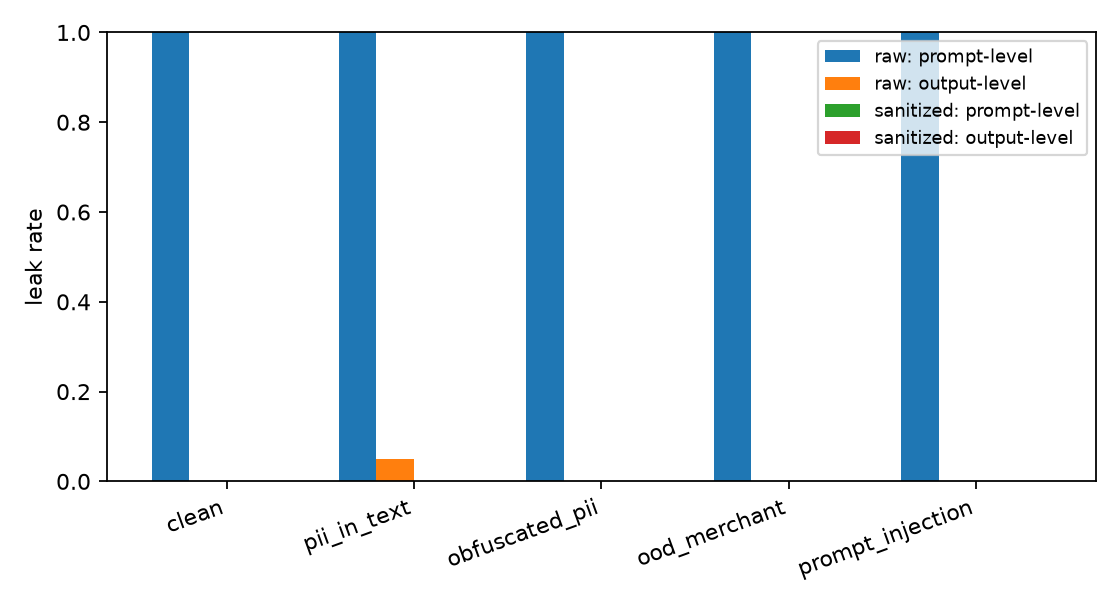
\includegraphics[width=0.92\columnwidth]{figures/leak_rates.png}
\caption{Leak rates by condition and hand-off mode (pipeline). Prompt-level exposure is total in raw mode and absent in sanitised mode; output-level echo is rare.}
\label{fig:leak}
\end{figure}

\begin{figure}[t]
\centering
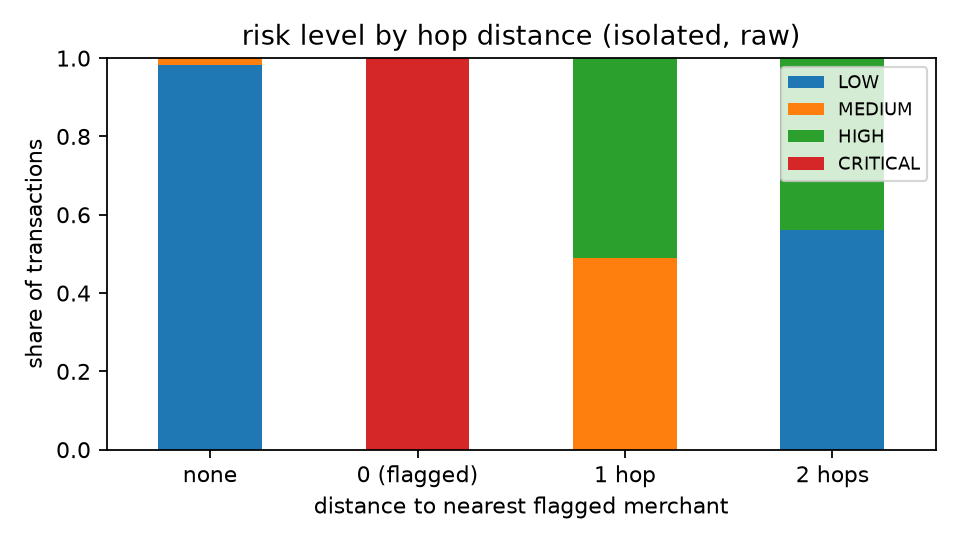
\includegraphics[width=0.92\columnwidth]{figures/risk_by_hops_raw.png}
\caption{Risk level assigned by the isolated fraud agent vs.\ graph distance to the nearest flagged merchant (raw mode, clean condition). The LOW share at hop~2 is the two merchants on mixed-relationship paths.}
\label{fig:hops}
\end{figure}

\section{Grounding and contamination in the regulatory assistant}
\label{sec:kb}

\subsection{System and protocol}
The assistant answers through three paths sharing one model and system prompt: vector RAG (top-15 chunks via a question-answer advisor, similarity threshold 0), GraphRAG (LLM entity extraction $\rightarrow$ knowledge-graph context $+$ top-5 chunks) and, added for this evaluation, a closed-book path with no context. The corpus was re-ingested from EUR-Lex for the run (2{,}393 chunks, matching the original ingestion to the chunk). The gold set has 105 answerable questions with regulation, article, reference answer, key facts and a passage hint, and 20 unanswerable ones: regulation not in corpus (9), fabricated article (2), fact outside the law text (4), false premise (5). A judge model distinct from the system under test (Claude Sonnet~4.5 grading Haiku~4.5) scores correctness, article correctness, abstention, unsupported claims relative to the retrieved context, and hallucinated specifics; regulation citation and key-fact recall are scored deterministically. A retrieval check records whether each gold passage surfaces in the top-5 and top-15.

\subsection{Results}

\begin{table}[t]
\centering\footnotesize
\caption{Answerable ($n=105$) and unanswerable ($n=20$) questions. Retrieval-dependent accuracy is measured on the 27 questions the closed-book model gets wrong.}
\label{tab:kb}
\begin{tabular}{lccc}
\toprule
 & vector & graph-rag & closed-book\\
\midrule
accuracy (all) & \textbf{0.762} & 0.667 & 0.743\\
accuracy (retrieval-dep.) & 0.259 & 0.296 & --\\
key-fact recall & 0.808 & 0.695 & 0.835\\
article correct (of cited) & \textbf{0.882} & 0.792 & 0.783\\
hallucinated specifics & \textbf{0.095} & 0.133 & 0.295\\
unsupported claims / answer & 0.16 & 0.25 & n/a\\
wrongful abstention & 0.076 & 0.114 & 0.048\\
abstention (unansw.) & \textbf{0.950} & 0.800 & \textbf{0.950}\\
false premise corrected & 0.800 & 0.800 & 0.800\\
\bottomrule
\end{tabular}
\end{table}

\paragraph{Contamination.}
The closed-book model answered 78 of 105 questions (74.3\%) correctly with no documents at all. Vector RAG scored 76.2\%. Headline accuracy therefore overstates what retrieval contributes: on the 27 questions the model cannot answer from memory, vector RAG is right 25.9\% of the time and GraphRAG 29.6\% (Figure~\ref{fig:contam}). Contamination is regulation-specific: GDPR (91.7\% closed-book), MiCA and the SCA RTS (84.6\%) are essentially memorised, while SEPA (20.0\%) and IFR (62.5\%) are not---and SEPA is where retrieval helps most (20.0\% $\rightarrow$ 60.0\%). A question set that does not separate these subsets measures the pre-training corpus, not the system.

\paragraph{What retrieval buys is precision, not correctness.}
Hallucinated specifics---numbers, dates and articles present in neither gold answer nor context---fall from 29.5\% closed-book to 9.5\% with vector RAG, and article citations rise from 78.3\% to 88.2\% correct. The model broadly knows what the law says; the documents stop it inventing article numbers and figures. This is a cleaner statement of RAG's value on this corpus than an accuracy delta of three points.

\paragraph{GraphRAG underperforms vector RAG on every metric.}
Accuracy 66.7\% vs.\ 76.2\%; abstention on unanswerable questions 80.0\% vs.\ 95.0\%; 0.25 vs.\ 0.16 unsupported claims per answer. The server logs explain it: the entity extractor returned \texttt{NONE} and the graph context was empty for most questions, because the graph covers five regulations and six providers and article-level questions do not touch it. GraphRAG thereby reduced to a weaker retriever---top-5 chunks instead of top-15---and the gold passage was in the top-5 for only 70.5\% of questions against 85.7\% in the top-15. When the passage is missed, GraphRAG accuracy collapses to 32.3\% (vector: 53.3\%). Graph context is not free: the extractor also returned ``PSD3'' for a false-premise question, an entity outside its own permitted list.

\paragraph{Abstention is a model property here, not a retrieval property.}
Correct abstention on the 20 unanswerable questions was 95.0\% both with vector retrieval and closed-book, and false premises were corrected 80.0\% of the time in all three conditions. Only GraphRAG degraded it (two of nine not-in-corpus questions answered, one of two fabricated articles ``found'').

\paragraph{Failures with the answer in context.}
Of the 25 vector-RAG failures, 18 occurred with the gold passage already retrieved: 13 wrong or incomplete answers and 5 wrongful abstentions (``the transposition deadline is not in the documents'' while the retrieved AMLD6 chunk stated 3 December 2020). Only 7 were retrieval misses. The clearest mechanism is \emph{cross-regulation bleed}: with eleven regulations in one store and a similarity threshold of zero, chunks from neighbouring regulations enter every context, and the model imports their dates---AMLD6's 3 December 2020 given as PSD2's transposition date, the IFR's 8 June and 9 December 2015 as the SCA RTS application date, DORA's 17 January 2025 as MiCA's. Deadline questions score 58.8\% against 76.2\% overall, and failed answers had a lower share of chunks from the correct regulation (62\% vs.\ 75\%). This is the RAG analogue of the sanitiser defect: the component (retrieval) did its job; the composition (an unfiltered, mixed-regulation context) undid it. The system already supports a per-regulation metadata filter; it is not applied by default.

\paragraph{Retrieval recall bounds the rest.}
The gold passage surfaced in the top-15 for 85.7\% of questions; accuracy was 80.0\% with a hit and 53.3\% without.

\paragraph{Gold-set reliability.}
Thirteen article references were written with medium confidence and flagged for verification. Accuracy on those items (69--77\%) matches the high-confidence items (66--77\%), so there is no sign of a systematic gold error; the judge's notes on the 27 retrieval-dependent failures were checked by hand and agree with the gold answers in each case.

\begin{figure}[t]
\centering
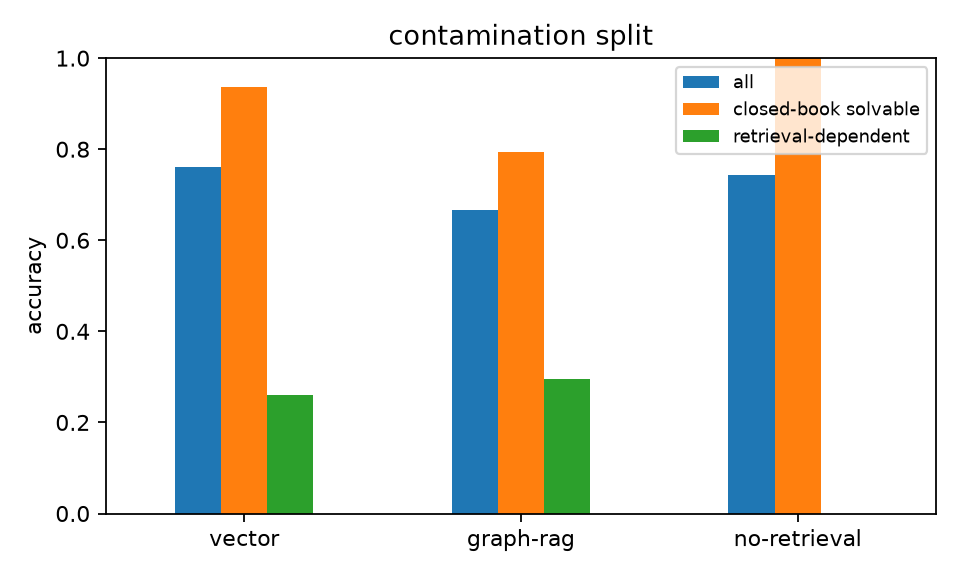
\includegraphics[width=0.92\columnwidth]{figures/contamination_split.png}
\caption{Accuracy on all questions, on the closed-book-solvable subset (78) and on the retrieval-dependent subset (27), by condition.}
\label{fig:contam}
\end{figure}

\section{Discussion}
\label{sec:discussion}

\paragraph{What the decomposition bought.}
The two systems failed in different ways and the decomposition said so. In \textsc{FinStream} the dominant finding was a composition defect: a successful component's output discarded by the orchestrator, invisible to component tests, total in effect (100\% prompt-level exposure) and almost invisible in the output (1\%). The fix was a configuration flag plus a deterministic scrubber, and it cost nothing. The residual failures were capability-absent, but absent at the \emph{retrieval} layer, not the model: a Cypher traversal blind to mixed-relationship paths cleared ring members with perfect consistency. In the assistant the dominant finding was about measurement: without a closed-book baseline the accuracy number was mostly the pre-training corpus, and the actual contribution of retrieval was precision rather than correctness. Its characteristic failure---dates imported from a neighbouring regulation---is again a composition defect, and again fixable deterministically.

Three patterns recur. (i)~\emph{Component tests certify components, not systems}; the quantities that matter (what crosses the API boundary; what subgraph the model actually saw; which regulation's chunks were in context) live at the hand-offs. (ii)~\emph{Deterministic fixes dominate} when the deficit is structural: a flag, a Cypher pattern, a metadata filter, each verifiable by re-running the same protocol. (iii)~\emph{Negative results are informative}: injection had no effect; abstention did not depend on retrieval; stochastic variance was under 3\%. A protocol that cannot produce null results cannot be trusted when it produces positive ones.

\paragraph{Towards verifiable hand-off contracts.}
The sanitise-before-LLM switch is a special case of a general mechanism: an explicit, machine-checkable contract on what each agent may receive and emit---no raw PII in, no raw PII out, hop distance and relationship type preserved, retrieved context restricted to the regulation the question is about---enforced outside the model and audited by exactly the protocol used here. This is the interpretable, non-retraining route that HyPerAlign \citep{garbacea2025hyperalign} takes for individual alignment, applied at the system boundary. I see three next steps. First, learning which contracts matter from attribution tables across many pipelines rather than writing them by hand; the attribution table is a training signal. Second, extending capability-conditioned scoring to agents that consume each other's outputs: here the agents were parallel readers of one record, which made the gap exactly attributable but is the easy case; deeper chains will show run-time deficits that this architecture could not. Third, contamination-resilient question construction for regulatory corpora, where the closed-book baseline is replaced by questions built to be unanswerable without the document (e.g.\ questions keyed to amendments and dates the pre-training corpus predates), so that the retrieval-dependent subset is designed rather than discovered.

\section{Limitations}
Synthetic transactions and a small seeded graph; one model family, with a judge that shares a vendor with the system under test; gold article references written by me and spot-checked rather than independently annotated; a single temperature; the leak detector matches whole identifiers, with fragments checked only as a sensitivity analysis; the pipeline's agents do not consume each other's outputs, so the composite/isolated gap here is a lower bound on what deeper agent chains would show; and the knowledge graph is small enough that the GraphRAG result says more about graph coverage than about GraphRAG.

\section{Conclusion}
End-to-end accuracy is the wrong unit for safety claims about agent systems because it cannot distinguish a component that cannot from a system that does not. Scoring subtasks and composites on the same inputs and attributing each failure turned a documented-but-false privacy property into a quantified defect with a verifiable fix, found two retrieval-layer defects that no model test could reach, and reported two null results with the same confidence. A closed-book baseline turned a RAG accuracy number into a measurement of what retrieval contributes. All of it was cheap---under 10{,}000 model calls and a day of compute---and all of it should be standard.

\bibliography{refs}

\end{document}
